\documentclass[10pt,conference,compsocconf]{IEEEtran}
\usepackage[T1]{fontenc}
\usepackage{newtxtext,newtxmath}
\usepackage{microtype}
\usepackage{graphicx}
\usepackage{booktabs}
\usepackage[hidelinks]{hyperref}
\newcommand{\paperauthors}{Jacobo Romero D\'iaz\textsuperscript{1}\qquad Pablo Gonz\'alez Monfort\textsuperscript{1}\qquad Roger Baiges Trilla\textsuperscript{1}}
\newcommand{\paperpdfauthors}{Jacobo Romero D\'iaz, Pablo Gonz\'alez Monfort, Roger Baiges Trilla}
\newcommand{\paperaffiliation}{\textsuperscript{1}\,EPFL, School of Computer and Communication Sciences}
\newcommand{\papercontact}{{\normalfont\mdseries\small\texttt{\{jacobo.romerodiaz, pablo.gonzalezmonfort, roger.baigestrilla\}@epfl.ch}}}

\hypersetup{pdftitle={Numerical Optimization and Nonlinear Models for Heart-Disease Classification},pdfauthor={\paperpdfauthors}}
\graphicspath{{figures/}}
\hyphenation{op-ti-mi-za-tion reg-u-lar-i-za-tion ques-tion-naire}

\begin{document}
\title{Numerical Optimization and Nonlinear Models\\
for Heart-Disease Classification}
\author{\paperauthors\\\paperaffiliation\\\papercontact}
\maketitle

\begin{abstract}
We study how data representation, numerical optimization, and model capacity
affect heart-disease classification in BRFSS survey responses. Under a
NumPy-only modeling constraint, we implement six linear and logistic methods,
investigate neural networks, and extend the comparison to gradient-boosted
trees. Encoding categories and missingness yields a strong logistic baseline;
greater neural capacity provides limited gains. Repeated cross-validation
favors boosted trees, while engineered features produce the highest recorded
F1 of 0.4474. We distinguish these local comparisons from the team's reported
public competition F1 of 0.456.
\end{abstract}

\section{Problem and Data Representation}
Our task is to classify self-reported coronary heart disease or myocardial
infarction (\texttt{\_MICHD}) from the 2015 Behavioral Risk Factor Surveillance
System (BRFSS)~\cite{cdc2015}. The course release contains 328,135 labeled
respondents, 109,379 test respondents, and 321 predictors. Only 8.83\% of
training labels are positive: predicting every respondent negative already
gives 91.17\% accuracy, but zero positive-class F1. We therefore prioritize F1
and use ROC AUC as a threshold-independent ranking measure.

\paragraph{Preserving questionnaire semantics}
Almost 45\% of entries are missing, often because a question is inapplicable
or belongs to an optional module. Numeric codes are not necessarily
quantities: \texttt{PHYSHLTH}=88 means zero days of poor physical health,
whereas 77 and 99 mean unknown and refused. Codebook-based rules remove
14 survey-design fields, two exact copies, and 14 mixed-unit fields with
computed replacements. We convert units and fill implied numeric skips,
leaving 56 numeric and 235 categorical predictors. Categorical unknown and
refused answers retain their identities.

\paragraph{A representation suited to linear models}
Numeric variables receive training-median imputation and missingness
indicators. Categorical levels observed at least 30 times are one-hot encoded,
with a separate missing category; rare or unseen levels map to all zeros.
Standardization yields approximately 1,530 columns. All learned statistics
are fitted within each training fold. Figure~\ref{fig:representation}
illustrates the importance of encoding; it is an exploratory diagnostic,
not the repeated-CV comparison below.

\begin{figure}[t]
  \centering
  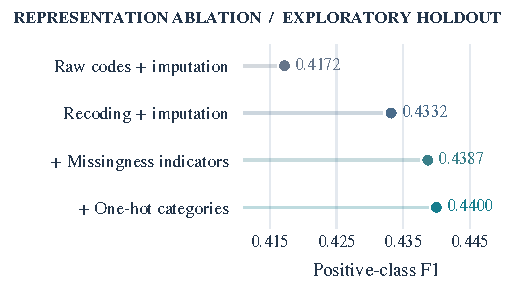
\includegraphics[width=\columnwidth]{representation.pdf}
  \caption{Exploratory logistic-regression ablation on one 80/20 split.
  F1 uses a validation-optimized threshold and is optimistic. Recoding also
  removes survey-design fields and maps categorical unknowns to missing;
  the final pipeline instead retains these categorical codes.}
  \label{fig:representation}
\end{figure}

\section{Numerical Methods and Model Capacity}\label{sec:methods}
\paragraph{Objectives and optimization}
For a design matrix $X$ including an intercept, labels $y\in\{0,1\}^N$,
and scores $z=Xw$, we minimize
\begin{align}
  L_{\mathrm{MSE}}(w)&=\frac{\lVert Xw-y\rVert_2^2}{2N},\\
  L_{\mathrm{log}}(w)&=\frac{1}{N}\sum_{i=1}^{N}
  \bigl[\log(1+e^{z_i})-y_i z_i\bigr].
\end{align}
Ridge and regularized logistic regression add $\lambda\lVert w\rVert_2^2$;
gradient descent (GD) updates $w\leftarrow w-\gamma\nabla L(w)$.
We compare MSE GD, single-sample stochastic GD (SGD), least squares, ridge,
logistic GD, and regularized logistic GD, all implemented in NumPy.

\paragraph{Conditioning and numerical stability}
One-hot dependencies make $X^\top X$ singular; least squares uses a
pseudoinverse and ridge solves $(X^\top X+2N\lambda I)w=X^\top y$.
The measured $\lambda_{\max}(X^\top X/N)\simeq63.3$ gives MSE GD's
stability condition $\gamma<2/63.3$. We use $\gamma=0.02$ for 100 steps,
and $\gamma=0.1$ for 300 logistic steps. SGD takes $10^6$ single-sample
updates at $\gamma=5\cdot10^{-6}$; rare standardized categories produce
large row norms. Both regularized presets use $\lambda=10^{-3}$.
Stable \texttt{logaddexp} evaluates logistic loss. MSE solvers share a
hypothesis class; finite budgets affect their numerical solutions.

\paragraph{Neural networks as a capacity test}
Exploratory multilayer perceptrons (MLPs) use one hidden ReLU layer, Adam
optimization~\cite{kingma2015adam}, and validation-based early stopping.
Widths 64 and 256 achieve holdout F1 of 0.4341 and 0.4402; the latter uses
dropout 0.3~\cite{srivastava2014dropout}. Reported overfitting after one to two
epochs motivates regularization rather than unbounded expansion. A later MLP
achieves repeated-CV F1 of 0.4399. These experiments test whether learned
nonlinear interactions improve on a well-encoded additive classifier;
the observed gains are limited.

\paragraph{A nonlinear extension with explicit interactions}
Motivated by gradient boosting~\cite{chen2016xgboost,ke2017lightgbm}, we implement
histogram trees in NumPy, with learned missing-value routing. A tuned ensemble
uses depth 5, 550 trees, learning rate 0.05, 64 bins, leaf penalty 10,
and row/feature fractions 0.7/0.3, averaging logits from model seeds 0--2.
A later variant uses 2,000 trees at rate 0.02 and adds eight response-count
features plus categorical target-rate encoding, smoothed with 50 pseudo-rows
at the training prevalence. Target statistics are learned only on training
folds. The five-member feature ensemble combines three seeds with two
additional variants: feature fraction 0.2 and minimum child Hessian 1.

\section{Evaluation and Results}
\paragraph{Protocol and decision threshold}
Table~\ref{tab:numerical} compares the six required methods on the same five
shuffled folds (seed 42), with thresholds optimized on each model's training
scores. The advanced comparison uses split seeds 42--44, five folds each;
each scored fold takes its threshold from the other folds' out-of-fold
predictions. Thresholds around 0.20--0.24 outperform the default 0.5 in this
imbalanced task. Hyperparameters and blend weights are selected using these
validation data, so this is not fully nested model-selection CV.

\begin{table}[t]
  \caption{Five-fold comparison of numerical methods. All rows except
  ``Raw inputs'' share the encoded design. Spread is fold standard deviation,
  not a confidence interval.}
  \label{tab:numerical}
  \centering
  \small
  \setlength{\tabcolsep}{5pt}
  \begin{tabular}{@{}lcc@{}}
\toprule
Method & F1 (mean $\pm$ SD) & AUC\\
\midrule
Raw inputs / LS & $0.4095 \pm 0.0019$ & 0.845 \\
MSE / GD & $0.4289 \pm 0.0022$ & 0.858 \\
MSE / SGD & $0.4255 \pm 0.0033$ & 0.855 \\
Least squares & $0.4301 \pm 0.0018$ & 0.857 \\
Ridge & $0.4297 \pm 0.0031$ & 0.858 \\
Logistic / GD & $\mathbf{0.4390} \pm 0.0027$ & 0.864 \\
L2 logistic / GD & $0.4388 \pm 0.0022$ & 0.864 \\
\bottomrule
\end{tabular}

\end{table}

\paragraph{Representation and loss matter before complexity}
For least squares, encoding increases F1 from 0.4095 to 0.4301.
Logistic GD reaches 0.4390 and improves on least squares on every fold;
the tested L2 penalty adds no benefit. The exploratory encoding sequence
in Fig.~\ref{fig:representation} supports preserving missingness and categories.
However, once one-hot encoding is present, numeric cleaning alone changes
paired five-fold F1 by only $-0.0003$; its semantic correctness should not be
confused with a measurable incremental gain.

\begin{figure}[t]
  \centering
  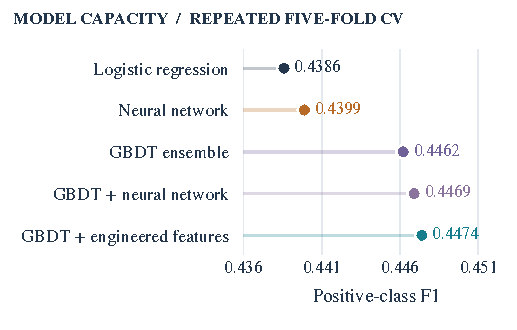
\includegraphics[width=\columnwidth]{model_families.pdf}
  \caption{Recorded means over 15 validation folds, with thresholds selected
  from other folds' OOF scores. Points are selected configurations; no error
  bars are inferred from unavailable fold records. The later MLP is a
  separate experiment from the exploratory networks in Section~\ref{sec:methods}.}
  \label{fig:families}
\end{figure}

\paragraph{Nonlinearity helps; the final increments are uncertain}
In the repeated comparison, logistic regression reaches 0.4386, the MLP
0.4399, and the tuned tree ensemble 0.4462 (AUC 0.8703).
The recorded Nadeau--Bengio corrected paired comparison~\cite{nadeau2003inference}
estimates a tree--logistic F1 gain of 0.0077, with a 95\% interval
$[0.0038,0.0115]$. Adding the MLP to the trees reaches 0.4469;
engineered features and ensembling reach 0.4474
(Fig.~\ref{fig:families}). The latter gain is only about 0.0011 over the
tuned ensemble (corrected $t=1.51$). These selected-model comparisons
support the larger tree gain more strongly than the final refinements;
they do not account for the full model search. The team's best reported
public AIcrowd F1 is 0.456, kept separate from the local CV results.

\section{Discussion and Reproducibility}
Our strongest finding is the progression from meaningful representation to
a well-optimized logistic baseline, then to a nonlinear model with a
larger measured gain. Extra neural capacity and ensemble diversity do not
automatically improve generalization. Importantly, all 773 training
respondents answering \texttt{HAREHAB1} are positive: this post-infarction
rehabilitation question~\cite{cdc2015} leaks diagnosis information. Retaining
it aids the benchmark but precludes interpreting the scores as prospective
clinical prediction.

Executable numerical methods, transforms, and GBDT recipes accompany this
report. Results come from archived summaries; MLP source and fold artifacts
are absent from this checkout. The current \texttt{run.py} refits the earlier
three-member ensemble. Linking the 0.456 submission to its exact configuration
and verifying identical predictions remain necessary for final reproducibility.

\clearpage
\IEEEtriggeratref{4}
\bibliographystyle{IEEEtran}
\bibliography{references}
\end{document}
